\documentclass[main.tex]{subfiles} % Subfile-Class

% ============================================================================== %
%                            Subfile document                                    %
% ============================================================================== %

\begin{document}

% Template

% ===================================
\section{Konzeption Energieversorgung}

In diesem Abschnitt wird sich mit der Energieversorgung des Pfadfinders
auseinandergesetzt. In einem ersten Schritt werden Anforderungen
zusammengestellt, dann verschiedene Konzepte kommentiert sowie sich am Ende für
ein Konzept entschieden.

% ===================================
\subsection*{Anforderungen}

\paragraph{Autonome Versorgung}
Das Fahrzeug muss autonom fahren können. Deshalb ist eine kabellose Speisung
des Gefährts unerlässlich. Die benötigte Spannung im Boardnetz hängt direkt mit
den eingesetzten Motoren und ihren Nennspannungen zusammen.

\paragraph{Boardnetz-Spannung}
Bauteilrecherchen haben ergeben, dass 24V-Akkus im benötigten Leistungsbereich
praktisch nicht mit geringem Gewicht erhältlich sind. Ein Benefit einer höheren
Boardnetzspannung ist, dass auf Bauteile und Motoren aus dem Industriellen
Umfeld zurückgegriffen hätte werden können. Da diese allerdings in jedem Fall
ebenfalls zu schwer sind, wird eine Boardnetzspannung von 24V ausgeschlossen.

\paragraph{Energiebedarf}
Tabelle~\ref{tab:Energiebedarf_Akku} zeigt eine überschlägige Rechnung zum
benötigten Leistungsbedarf einzelner Teilgruppen. Zusätzliche 25\% Toleranz
geben den voraussichtlichen Energiebedarf des Gerätes mit $\approx 55W$ an.

\begin{table}[h!]
    \centering
    \begin{tabular}{|l|l|l|l|}
        \hline
        \textbf{Komponente}         & \textbf{P [W]} & \textbf{Anzahl} & \textbf{P total [W]} \\ \hline
        Schrittmotor                & 12             & 2               & 24                   \\ \hline
        Raspberry Pi 5              & 8.6            & 1               & 8.6                  \\ \hline
        RTC \& Sensoren             & 10             & 1               & 10                   \\ \hline
        Summe                       &                &                 & 42.6                 \\ \hline
        Summe inkl. 25\% Sicherheit &                &                 & 53.25                \\ \hline
    \end{tabular}
    \caption{Überschlagsrechnung zum Energiebedarf}~\label{tab:Energiebedarf_Akku}
\end{table}

\paragraph{Gewicht} Da das Gewicht des Fahrzeuges mit $2 kg$ stark beschränkt ist, darf das
Akkupaket nicht mehr als $ 0.5 kg$ wiegen.

\paragraph{Strombelastbarkeit}
Aus dem Leistungsbedarf ergibt sich eine minimale Strombelastbarkeit der
Akkumulatoren wie folgt:
\[
    I_{discharge} = \frac{P}{U_{Bat}}
\]
Für die Batterien ergeben sich also mindestens $4.6 A$ Strombelastbarkeit für
die Batterien.

% ===================================
\subsection{Konzeption}

Das Gewicht ist eine Grosse Einschränkung in der Entwicklung des Geräts.
Aufgrund seiner hohen Energiedichte werden lediglich Lithium-Ionen sowie
Lithium-Polymer betrachtet.

% ====== ##############################################################################################################
\subsubsection{Konzept 1 - 12V LiIon Akku - Eigenentwicklung}

Abbildung~\ref{fig:Konzept_12V_Eigenentw} zeigt ein Blockschaltbild dieser
Variante. Im folgenden Unterabschnitt werden die einzelnen Unterbaugruppen kurz
kommentiert.

\begin{figure}[h!]
    \centering
    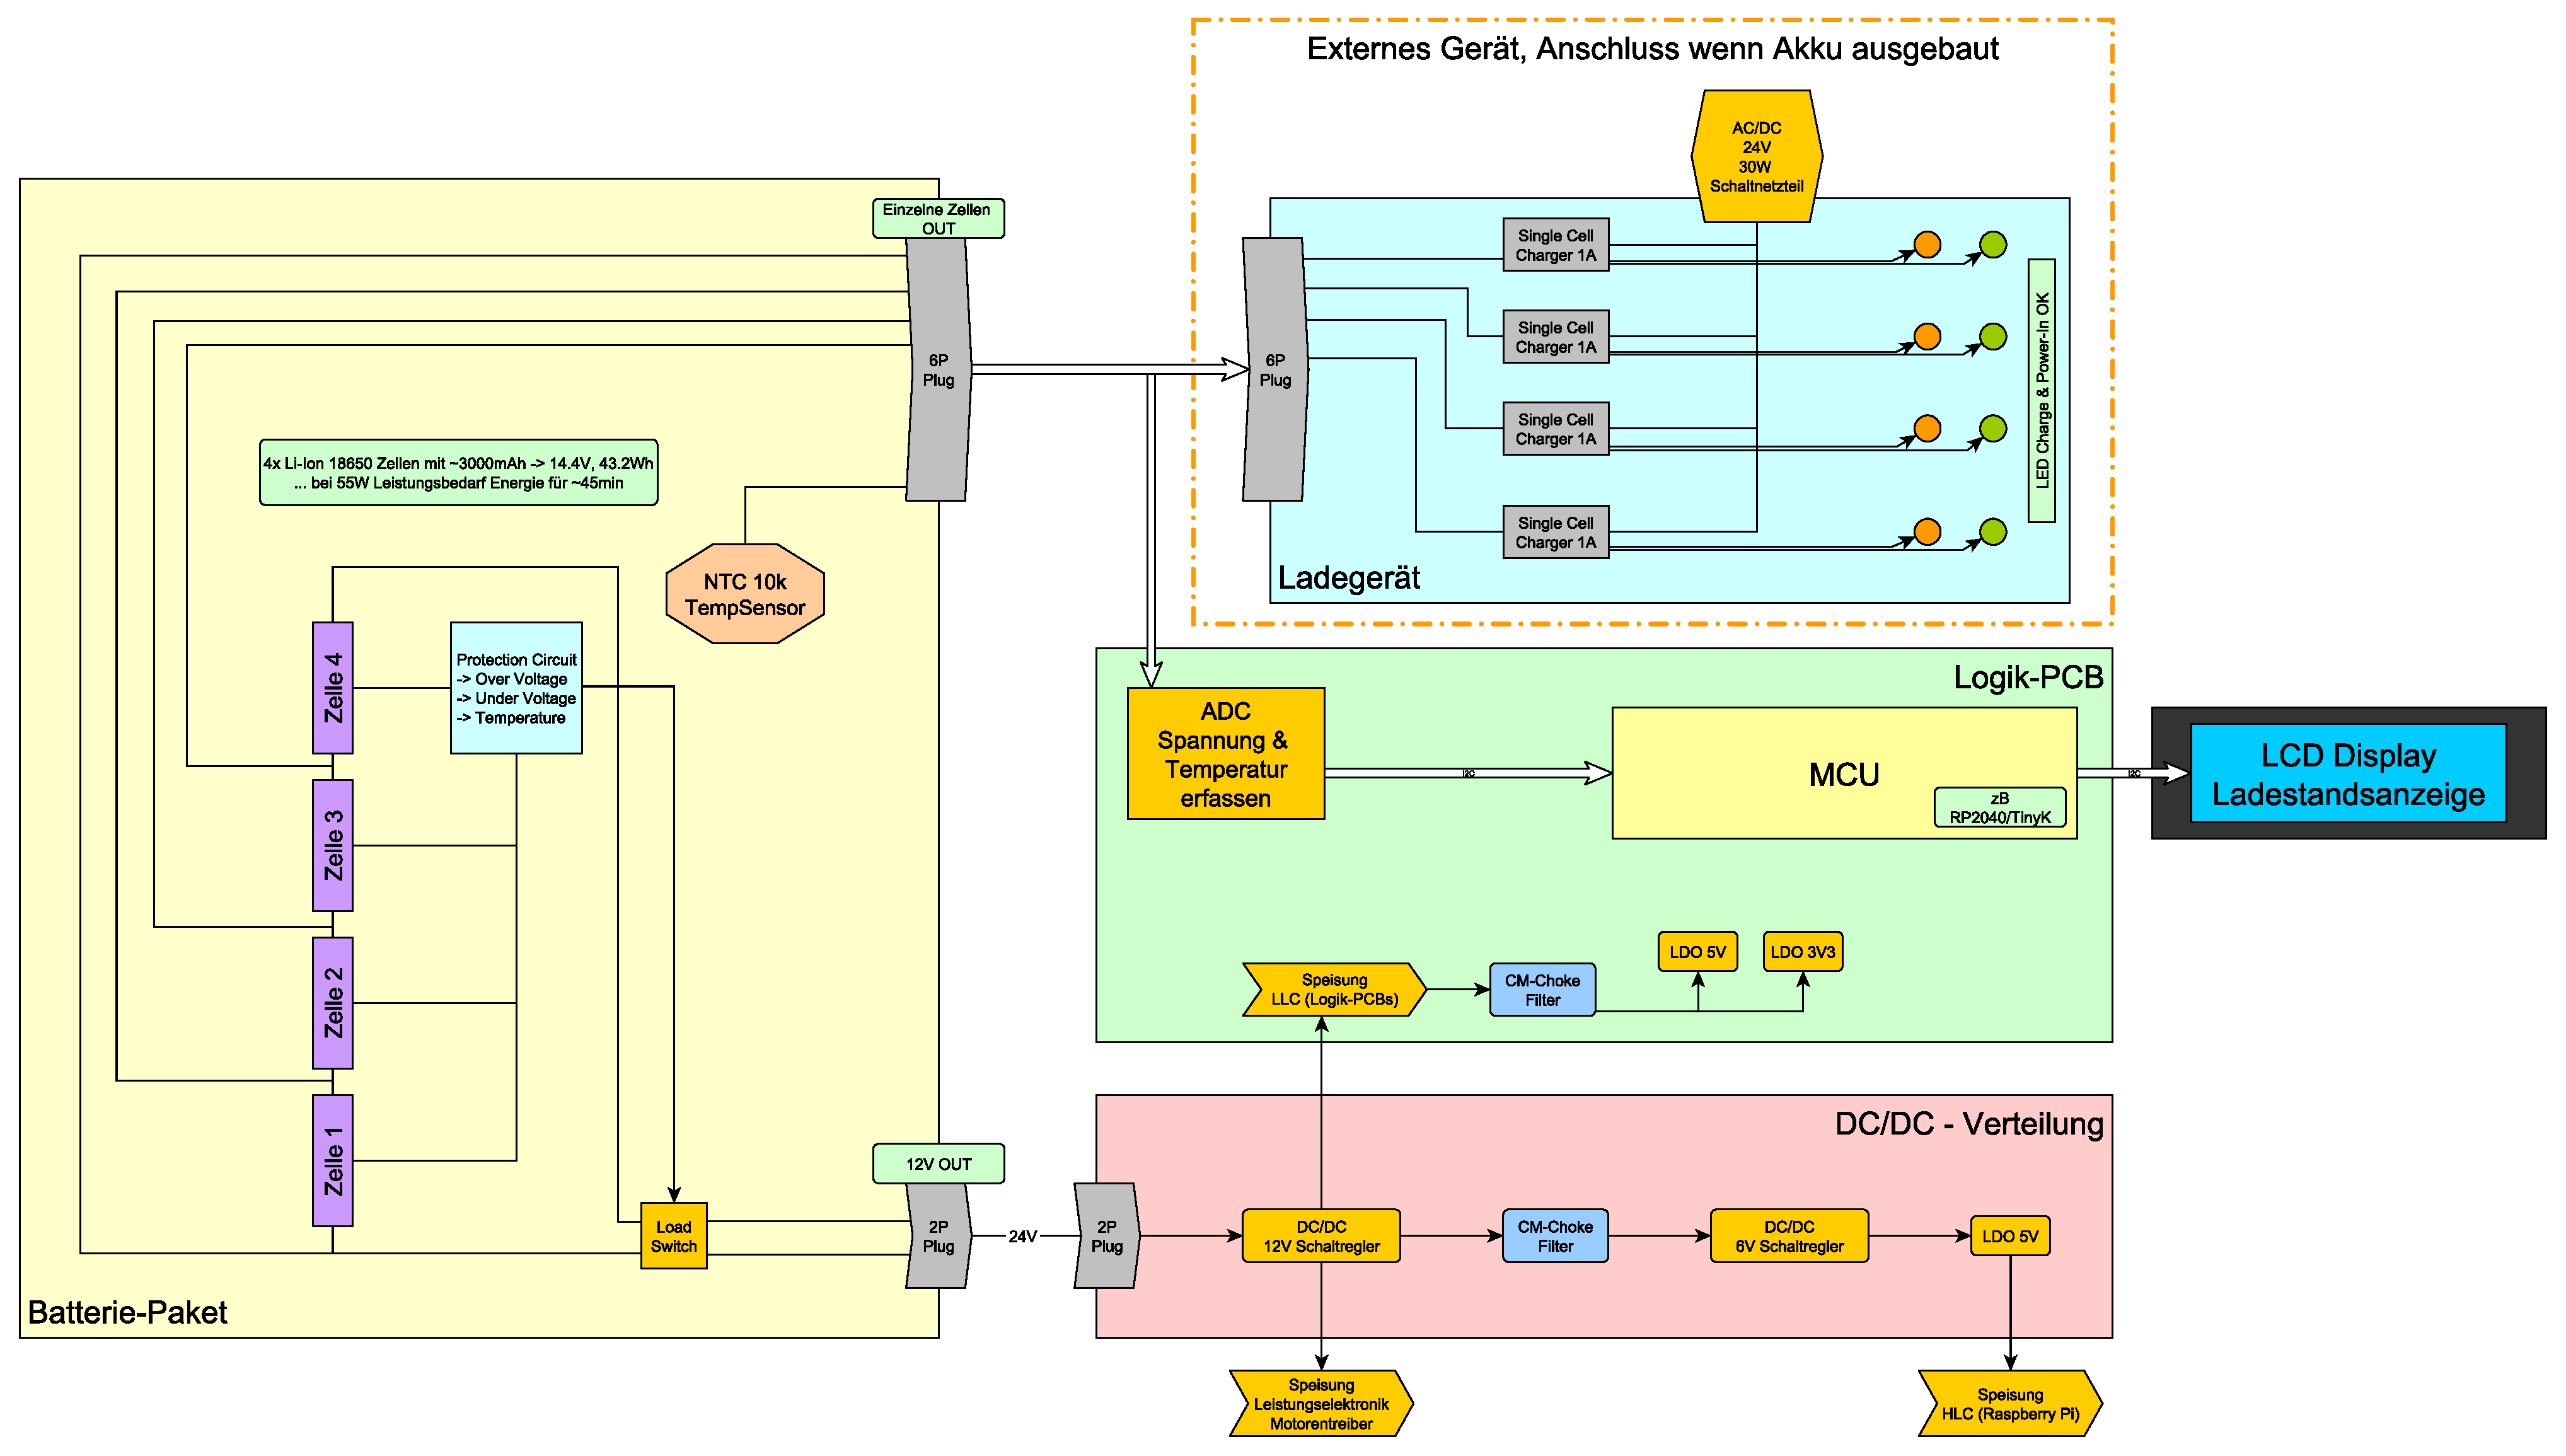
\includegraphics[width=1\textwidth]{./fig_Boardnetz/SpeisungsKonzept_LiIon_12V.pdf}
    \caption{Blockschaltbild des Akku-Konzepts 12V Variante}~\label{fig:Konzept_12V_Eigenentw}
\end{figure}

\paragraph{Akkuzelle}
Es sind 4 Lithium-Ionen Zellen der Bauform 18650 in Reihe geschaltet, um die
gewünschte Spannung zu erreichen. Diese Bauform ist in der Industrie gängig
vertreten und entsprechend einfach erhältlich. Die Nennspannung ergibt sich zu
$4 \cdot 3.6V = 14.4V$.

Die Akkuzelle enthält
\[
    E_{bat} = 4 \cdot 3.6V \cdot 3Ah = 43.2Wh
\]
Energie, die für einen Betrieb von ca. 45 Minuten ausreichen würde.

Mit einem DC/DC-Abwärtssteller werden daraus die benötigten 12V generiert.
Lithium-Ionen-Akkus benötigen eine Schutzbeschaltung, um sie vor Unter- oder
Überspannung zu schützen. Diese Ereignisse führen nicht nur zu Schäden an der
Akkuzelle selbst, sondern auch zum Entflammen des Akkupakets. Dazu ist auf dem
Akkupaket selbst ein IC der Firma Texas-Industries verbaut, welcher mit MOSFETS
den Akku von der Last trennen kann, falls sich die Spannung einem gefährlichen
Bereich nähern würde. Die Schutzbeschaltung wird auf dem Akku selbst
vorgesehen, damit sich Ladegerät und Roboter dieselbe Schutzbeschaltung teilen
können.

Das Gewicht dieses Akkupakets beläuft sich auf $\approx 320 g$, wie
Tabelle~\ref{tab:gewicht_12V_Eigenentw} zeigt. Hier könnte allergings noch am
Gewicht des Gehäuses gespart werden.

\begin{table}[h!]
    \centering
    \scriptsize % Schriftgröße verkleinern
    \begin{tabularx}{0.75\textwidth}{|>{\raggedright\arraybackslash}X|>{\raggedright\arraybackslash}p{0.8cm}|>{\centering\arraybackslash}p{0.8cm}|>{\centering\arraybackslash}p{0.8cm}|}
        \hline
        \textbf{Beschreibung}                    & \textbf{n} & \textbf{[g]} & \textbf{$\sum$ [g]} \\ \hline
        Batteriezelle                            & 4          & 30           & 120                 \\ \hline
        PCB 4 Lagen @100x100mm                   & 1          & 60           & 60                  \\ \hline
        Kleinmaterial (Stecker, IC's, Schrauben) & 1          & 15           & 10                  \\ \hline
        Gehäuse                                  & ~          & ~            & 100                 \\ \hline
        SUMME Battery Pack + 10\%                & ~          &              & $\approx 320g$      \\ \hline
    \end{tabularx}
    \caption{Gewichtsschätzung eines Akku-Pakets 12V Variante}~\label{tab:gewicht_12V_Eigenentw}
\end{table}

\paragraph{Kostenschätzung}
Um dieses Konzept bezüglich seiner Kosten bewerten zu können, ist ebenfalls
wieder eine Kostenabschätzung erstellt worden. Sie gleicht im Wesentlichen der
Schätzung aus der 24V-Variante: Es ist lediglich die Anzahl Zellen verringert,
sowie ein anderer Schutz-IC eingeplant worden. Die Kostenschätzungen sind
Tabelle~\ref{tab:Kostenschaetzung_12V_Akku} und
Tabelle~\ref{tab:Kostenschaetzung_12V_Ladegeraet} zu entnehmen.

\begin{table}[h!]
    \centering
    \scriptsize % Schriftgröße verkleinern
    \begin{tabularx}{\textwidth}{|>{\raggedright\arraybackslash}p{3cm}|>{\raggedright\arraybackslash}p{2cm}|>{\raggedright\arraybackslash}p{3cm}|>{\raggedright\arraybackslash}p{1.75cm}|>{\centering\arraybackslash}p{0.75cm}|>{\centering\arraybackslash}p{0.7cm}|>{\centering\arraybackslash}p{0.7cm}|}
        \hline
        \textbf{Beschreibung}            & \textbf{Hersteller} & \textbf{Hersteller Nr.} & \textbf{Distributor} & \textbf{n} & \textbf{CHF} & \textbf{$\sum$ CHF} \\ \hline
        Batteriezelle                    & Tenpower            & INR18650-32HE           & Nikon.nl             & 4          & 2.35         & 9.4                 \\ \hline
        Batteriezellenhalter             & MPD                 & BK-18650-CLIP           & Digikey              & 8          & 0.458        & 3.66                \\ \hline
        NTC Temperaturfühler             & Vishay Dale         & CRCW080510K0JNTC        & Digikey              & 1          & 0.12         & 0.12                \\ \hline
        MOSFET Leistungsschalter P-Kanal & Diodes Incorporated & DMP3036SFV-13           & DigiKey              & 2          & 0.55         & 1.1                 \\ \hline
        MOSFET Gate Treiber N-Kanal      & Nexperia USA Inc.   & 2N7002NXAKR             & DigiKey              & 2          & 0.09         & 0.18                \\ \hline
        Battery Protection IC            & Texas Instruments   & BQ296907DSGR            & Digikey              & 1          & 0.33         & 0.33                \\ \hline
        6P Stecker                       & TE                  & 2350514-6               & Digikey              & 1          & 0.83         & 0.83                \\ \hline
        2P Stecker                       & Würth Elektronik    & 691321300002            & Digikey              & 1          & 0.3          & 0.3                 \\ \hline
        Kleinmaterial (R's, C's, L's, …) & ~                   & ~                       & ~                    & 1          & 3            & 3                   \\ \hline
        PCB 4 Lagen @100x100mm           & ~                   & ~                       & JLCPCB               & 1          & 8            & 8                   \\ \hline
        Gehäuse                          & ~                   & ~                       & 3D Druck, leicht     & ~          & ~            & 0                   \\ \hline
        ~                                & ~                   & ~                       & ~                    & ~          & ~            & ~                   \\ \hline
        Versandpauschale                 & ~                   & ~                       & ~                    & 1          & 10           & 10                  \\ \hline
        SUMME Battery Pack + 10\%        & ~                   & ~                       & ~                    &            &              & 40.61               \\ \hline
    \end{tabularx}
    \caption{Kostenschätzung des Akku-Pakets 12V Variante}~\label{tab:Kostenschaetzung_12V_Akku}
\end{table}

\begin{table}[h!]
    \centering
    \scriptsize % Schriftgröße verkleinern
    \begin{tabularx}{\textwidth}{|>{\raggedright\arraybackslash}p{3cm}|>{\raggedright\arraybackslash}p{2cm}|>{\raggedright\arraybackslash}p{3cm}|>{\raggedright\arraybackslash}p{1.75cm}|>{\centering\arraybackslash}p{0.75cm}|>{\centering\arraybackslash}p{0.7cm}|>{\centering\arraybackslash}p{0.7cm}|}
        \hline
        \textbf{Beschreibung}             & \textbf{Hersteller}   & \textbf{Hersteller Nr.} & \textbf{Distributor} & \textbf{n} & \textbf{CHF} & \textbf{$\sum$ CHF} \\ \hline
        Ladegerät IC                      & 3Peak                 & TPB4056A20-ES1R         & DigiKey              & 4          & 0.17         & 0.68                \\ \hline
        LEDs Ladegerät                    & generisch 3mm         & ~                       & Digikey              & 8          & 0.15         & 1.2                 \\ \hline
        AC/DC Wandler Ladegerät           & Mean Well USA         & 1866-3343-ND            & DigiKey              & 1          & 11.44        & 11.44               \\ \hline
        6P Buchse                         & TE Connectivity       & 2350398-6               & DigiKey              & 1          & 3.93         & 3.93                \\ \hline
        Gehäuse                           & Hammond Manufacturing & 1455N1601               & Reichelt             & 1          & 17.8         & 17.8                \\ \hline
        Kleinmaterial  (R's, C's, L's, …) & ~                     & ~                       & ~                    & 1          & 3            & 3                   \\ \hline
        PCB 2 Lagen @100x100mm            & ~                     & ~                       & JLCPCB               & 1          & 8            & 8                   \\ \hline
        Versandpauschale                  & ~                     & ~                       & ~                    & 1          & 10           & 10                  \\ \hline
        SUMME Ladegerät +10\%             & ~                     & ~                       & ~                    &            &              & 61.655              \\ \hline
    \end{tabularx}
    \caption{Kostenschätzung des Ladegeräts der 12V Variante}~\label{tab:Kostenschaetzung_12V_Ladegeraet}
\end{table}

\paragraph{Strombelastbarkeit}
Die Akkuzellen sind belastbar mit einem Entladestrom von $8A$, was vollkommen
ausreichend ist für diese Anwendung.

\paragraph{Ladegerät}
Um die Akkuzelle zu laden, muss auch ein Ladegerät entwickelt werden. Dieses
wird mit ICs der Firma 3-Peak realisiert, welche jede Akkuzelle einzeln auf
4.2V mit einem konstanten Strom von $1A$ lädt. Dadurch, dass jede Zellen über
ein eigenes Ladegerät verfügt, werden die Zellen auch bereits bei jedem
Ladevorgang balanciert. Versorgt werden diese einzelnen Ladegeräte über ein
AC-DC-Schaltnetzteil, welches 5W zur Verfügung stellt.

Die benötigte Leistung berechnet sich wie folgt:
\[
    P_{crg} = 4 \cdot I_{crg} \cdot U_{crg} =  4 \cdot 1A \cdot 4.2V = 16.8W
\]

Das Ladegerät ist nicht teil des Geräts und wird deshalb nicht in seinem
Gewicht beurteilt.

\paragraph{Akku Monitoring}
Die Anforderungsliste des Pfadfinders sieht vor, den Ladezustand des Akkus über
ein LCD-Display darzustellen. Um dies zu ermöglichen, werden die einzelnen
Zellenanschlüsse nochmals separat herausgeführt, um sie auf dem Pfadfinder
selbst mit einem ADC auswerten und entsprechend anzeigen zu können.

% ====== ##############################################################################################################
\subsubsection{Konzept 2 - 12V LiPo Akku - Kaufteil}

Eine Akkuzelle muss nicht zwingend selbst entwickelt werden. Aus dem
Modellbau-Bereich kann aus einer breiten Palette ein passender Akku ausgewählt
und eingesetzt werden. Ein günstiger Anbieter dieser Akku-Pakete ist die Firma
\textit{Swaytronic}. Dieser Hersteller bietet nicht nur Akkumulatoren an,
sondern auch Lösungen, wie diese aufgeladen werden können. In den Parametern
Gewicht, Kapazität und Baugrösse bewegen sich die meisten Hersteller in einem
ähnlichen Rahmen, weshalb hier auf Akkus der Firma \textit{Swaytronic}
stellvertretend für alle Modellbau-Akkuhersteller eingegangen wird.

\paragraph{Akkuzelle}

Mit sogenannten 4S-Akkupacks erhält man eine Nennspannung von
\[
    U_{bat} = 4 \cdot 3.6V = 14.4V
\]
Um diese Akkupakete mit den Eigenentwicklungen vergleichen zu können, wird in
einem ähnlichen Kapazitätsbereich von $3000mAh$ geschaut. Diese Akkupacks haben
praktisch den gleichen Energieinhalt wie die Eigenentwicklung mit $43.2Wh$.
Herausgesucht wurde der Akku \textit{SWAY-EL LiPo 4S 14.8V 3000mAh 35C/70C EC3
} von \textit{Swaytronic}, abgebildet in
Abbildung~\ref{fig:Swaytronic_4S_Akkupack}. Die Schutzbeschaltung wird auch
hier auf dem Pfadfinder umgesetzt werden müssen, da die Akkus eine solche nicht
integriert haben. Zugriff auf die Zellspannungen erhält man über den separat
herausgeführten Steckverbinder, welcher eben genau diese Anschlüsse
bereitstellt.

\paragraph{Kostenschätzung}

Die Akkuzelle beläuft sich auf den in
Tabelle~\ref{tab:Kostenschaetzung_12V_Akku_kaufteile} berechneten Preis. Die
Kosten für das Ladegerät kann
Tabelle~\ref{tab:Kostenschaetzung_24V_Ladegeraet_kaufteile} entnommen werden.

\begin{table}[h!]
    \centering
    \scriptsize % Schriftgröße verkleinern
    \begin{tabularx}{\textwidth}{|>{\raggedright\arraybackslash}p{3cm}|>{\raggedright\arraybackslash}p{2cm}|>{\raggedright\arraybackslash}p{3cm}|>{\raggedright\arraybackslash}p{1.75cm}|>{\centering\arraybackslash}p{0.75cm}|>{\centering\arraybackslash}p{0.7cm}|>{\centering\arraybackslash}p{0.7cm}|}
        \hline
        \textbf{Beschreibung}            & \textbf{Hersteller} & \textbf{Hersteller Nr.} & \textbf{Distributor} & \textbf{n} & \textbf{CHF} & \textbf{$\sum$ CHF} \\ \hline
        Batteriepaket                    & Swaytronic          & 7640182625344           & Swaytronic.ch        & 1          & 58.35        & 58.35               \\ \hline
        MOSFET Leistungsschalter P-Kanal & Diodes Incorporated & DMP3036SFV-13           & DigiKey              & 2          & 0.55         & 1.1                 \\ \hline
        MOSFET Gate Treiber N-Kanal      & Nexperia USA Inc.   & 2N7002NXAKR             & DigiKey              & 2          & 0.09         & 0.18                \\ \hline
        Battery Protection IC            & Texas Instruments   & BQ296907DSGR            & Digikey              & 1          & 0.33         & 0.33                \\ \hline
        Steckverbinder Pauschale         &                     &                         &                      & 2          & 1.5          & 3                   \\ \hline
        Kleinmaterial (R's, C's, L's, …) & ~                   & ~                       & ~                    & 1          & 3            & 3                   \\ \hline
        Gehäuse                          & ~                   & ~                       & 3D Druck, leicht     & ~          & ~            & 0                   \\ \hline
        ~                                & ~                   & ~                       & ~                    & ~          & ~            & ~                   \\ \hline
        Versandpauschale                 & ~                   & ~                       & ~                    & 1          & 10           & 10                  \\ \hline
        SUMME Battery Pack + 10\%        & ~                   & ~                       & ~                    &            &              & 83.56               \\ \hline
    \end{tabularx}
    \caption{Kostenschätzung des Akku-Pakets 12V Variante mit Kaufteilen}~\label{tab:Kostenschaetzung_12V_Akku_kaufteile}
\end{table}

\begin{table}[h!]
    \centering
    \scriptsize % Schriftgröße verkleinern
    \begin{tabularx}{\textwidth}{|>{\raggedright\arraybackslash}p{3cm}|>{\raggedright\arraybackslash}p{2cm}|>{\raggedright\arraybackslash}p{3cm}|>{\raggedright\arraybackslash}p{1.75cm}|>{\centering\arraybackslash}p{0.75cm}|>{\centering\arraybackslash}p{0.7cm}|>{\centering\arraybackslash}p{0.7cm}|}
        \hline
        \textbf{Beschreibung} & \textbf{Hersteller} & \textbf{Hersteller Nr.} & \textbf{Distributor} & \textbf{n} & \textbf{CHF} & \textbf{$\sum$ CHF} \\ \hline
        Ladegerät             & Swaytronic          & 7640159368274           & Swaytronic.ch        & 1          & 73.15        & 73.15               \\ \hline
    \end{tabularx}
    \caption{Kostenschätzung des Ladegeräts 12V Variante mit Kaufteilen}~\label{tab:Kostenschaetzung_24V_Ladegeraet_kaufteile}
\end{table}

% ====== ##############################################################################################################
\subsubsection{Konzept 3 - 12V LiPo Akku - Kaufteil mit weniger Kapazität}

Dieses Akkupaket besitzt eine geringere Kapazität. Für eine Betriebsdauer von
$\approx 15 min $ würde ein Energiegehalt von $13.75Wh$ bereits ausreichen. Für
einen 4S-Akku sind das in etwa $1000 mAh$.

\paragraph{Akkuzelle}

Das Akkupack \textit{SWAY-FPV LiPo 4S 14.8V 1000mAh 60C/120C XT60} ist mit 115g
und 25.55 CHF ein bezahlbares und vergleichsweise leichtes Modell mit
ausreichender Akkukapazität.

\paragraph{Kostenschätzung}

Die Akkuzelle beläuft sich auf den in
Tabelle~\ref{tab:Kostenschaetzung_12V_Akku_kaufteile_wenigerKap} berechneten
Preis. Die Kosten für das Ladegerät kann
Tabelle~\ref{tab:Kostenschaetzung_24V_Ladegeraet_kaufteile} entnommen werden.

\begin{table}[h!]
    \centering
    \scriptsize % Schriftgröße verkleinern
    \begin{tabularx}{\textwidth}{|>{\raggedright\arraybackslash}p{3cm}|>{\raggedright\arraybackslash}p{2cm}|>{\raggedright\arraybackslash}p{3cm}|>{\raggedright\arraybackslash}p{1.75cm}|>{\centering\arraybackslash}p{0.75cm}|>{\centering\arraybackslash}p{0.7cm}|>{\centering\arraybackslash}p{0.7cm}|}
        \hline
        \textbf{Beschreibung}            & \textbf{Hersteller} & \textbf{Hersteller Nr.} & \textbf{Distributor} & \textbf{n} & \textbf{CHF} & \textbf{$\sum$ CHF} \\ \hline
        Batteriepaket                    & Swaytronic          & 7640182620677           & Swaytronic.ch        & 1          & 25.55        & 25.55               \\ \hline
        MOSFET Leistungsschalter P-Kanal & Diodes Incorporated & DMP3036SFV-13           & DigiKey              & 2          & 0.55         & 1.1                 \\ \hline
        MOSFET Gate Treiber N-Kanal      & Nexperia USA Inc.   & 2N7002NXAKR             & DigiKey              & 2          & 0.09         & 0.18                \\ \hline
        Battery Protection IC            & Texas Instruments   & BQ296907DSGR            & Digikey              & 1          & 0.33         & 0.33                \\ \hline
        Steckverbinder Pauschale         &                     &                         &                      & 2          & 1.5          & 3                   \\ \hline
        Kleinmaterial (R's, C's, L's, …) & ~                   & ~                       & ~                    & 1          & 3            & 3                   \\ \hline
        Gehäuse                          & ~                   & ~                       & 3D Druck, leicht     & ~          & ~            & 0                   \\ \hline
        ~                                & ~                   & ~                       & ~                    & ~          & ~            & ~                   \\ \hline
        Versandpauschale                 & ~                   & ~                       & ~                    & 1          & 10           & 10                  \\ \hline
        SUMME Battery Pack + 10\%        & ~                   & ~                       & ~                    &            &              & 47.47               \\ \hline
    \end{tabularx}
    \caption{Kostenschätzung des Akku-Pakets 12V Variante mit Kaufteilen}~\label{tab:Kostenschaetzung_12V_Akku_kaufteile_wenigerKap}
\end{table}

% ====== ##############################################################################################################

\subsubsection{Fazit und Entscheidung der Konzeptphase}

Tabelle~\ref{tab:Vergleich_Akkukonzepte} zeigt einen Vergleich der
verschiedenen Konzepte, um sie direkt miteinander gegenüberstellen zu können.

\begin{table}[!ht]
    \centering
    \scriptsize % Schriftgröße verkleinern
    \begin{tabularx}{\textwidth}{|>{\raggedright\arraybackslash}X|>{\centering\arraybackslash}p{1.5cm}|>{\centering\arraybackslash}p{1.5cm}|>{\centering\arraybackslash}p{1.5cm}|>{\centering\arraybackslash}p{1.5cm}|>{\centering\arraybackslash}p{1.5cm}|}
        \hline
        \textbf{Kriterium}         & \textbf{Konzept 1} & \textbf{Konzept 2} & \textbf{Konzept 3} \\ \hline
        Enthaltene Energie [Wh]    & 42.2               & 44.4               & 32.56              \\ \hline
        Betriebsdauer [min]        & 40                 & 45                 & 30                 \\ \hline
        Boardnetzspannung [V]      & 12                 & 12                 & 12                 \\ \hline
        Maximaler Entladestrom [A] & 8                  & 105                & 77                 \\ \hline
        Gewicht [g]                & 310                & 300                & 235                \\ \hline
        Kosten Akkupack [CHF]      & 40                 & 83                 & 66                 \\ \hline
        Kosten Ladegerät  [CHF]    & 60                 & 73                 & 73                 \\ \hline
        Kosten Total  [CHF]        & 100                & 156                & 139                \\ \hline
    \end{tabularx}
    \caption{Vergleichstabelle der verschiedenen Konzepte}~\label{tab:Vergleich_Akkukonzepte}
\end{table}

In einer gemeinsamen Sitzung ist der Entscheid auf das Konzept 3 gefallen.
Hauptargumente sind der etwas reduzierte Entwicklungsaufwand, der günstige
Preis für eine angemessene Kapazität sowie ein geringes Gewicht. Bei eben
dieser Besprechung hat sich ebenfalls der Wunsch an eine Möglichkeit ergeben,
den Pfadfinder auch über ein externes Netzteil speisen zu können. Dadurch
entschärft sich ebenfalls die geringere Akkukapazität, da das Gerät bei
Einrichttätigkeiten oder Versuchen nicht zwingend vom Akkubetrieb abhängig sein
wird. Es kann in solchen Fällen dann auch stationär an einem Arbeitsplatz über
ein Netzkabel betrieben werden.

% ===================================
\subsection{Entwicklung und Dimensionierung}

Entwickelt wird eine Schaltung, welche die Akkuspannung im Netz verteilen kann,
sowie eine gewisse Schutzbeschaltung für den Akku bietet. Nachfolgend sind
Anforderungen an diese Schaltung aufgeführt.

\subsubsection{Anforderungen}
\begin{description}
    \item[Schutz vor Über-/ Unterspannung] Die verwendete Akkutechnologie kann in Brand
          geraten, falls der Akku ausserhalb seines sicheren Arbeitsbereichs betrieben
          wird. Eine entsprechende Schutzbeschaltung muss also zwingend vorgesehen
          werden.
    \item[Quellenumschaltung] Die Schaltung muss automatisch, sobald ein Netzteil
          angehängt wird, die Batterie vom Boardnetz trennen. Die verwendete
          Spannungsquelle kann optisch über eine LED signalisiert werden.
    \item[Einschaltstrombegrenzung] Im gesamten Schaltkreis befinden sich Kapazitäten.
          Der Einschaltstrom muss daher begrenzt werden.
    \item[Akkuzellenüberwachung] Aus der Anforderungsliste des Gesamtgeräts ergibt sich,
          dass die einzelnen Zellen überwacht werden sollen.
    \item[Ein- und Abschalten] Über einen Schalter muss die Spannungsversorgung des
          Geräts abgeschaltet werden können. Der Betriebszustand kann optisch über eine
          LED dargestellt werden.
    \item[Anzahl der Ausgänge] Die Schaltung muss genügend Ausgänge bieten, um jegliche
          Elektronik auf dem Gerät anschliessen zu können. Dabei soll ein in der
          Industrie üblicher, einfacher Steckverbinder eingesetzt werden.
    \item[Verpolungsschutz] Der Anschluss soll einen Verpolungsschutz sowohl beim
          Netzteilanschluss als auch beim Batterieanschluss bieten. Verpolte Anschlüsse
          sind anzuzeigen, dies kann zum Beispiel optisch über eine LED erfolgen.
\end{description}

% ====================================================================================
\subsubsection{Schaltungsbeschreibung}

\paragraph{Batterieschutz}
Als Batterieschutz-IC wird der \textit{BQ7790400PWR} der Firma Texas-Industries
eingesetzt. Dieser bitetet die Funktion, bei Detektierter Unterspannung einer
Batteriezelle einen MOSFET abzuschalten, womit die Batterie vom Netz getrennt
wird. Im Schema schaltet der IC \textit{U401} also die beiden MOSFETS
\textit{Q203} und \textit{Q205}. Zweiterer ist lediglich dafür da, eine LED zu
schalten falls eine Unterspannung detektiert wird. Der Ausgang des IC's kann
nicht sonderlich viel Strom treiben, weshalb für diese LED ebenfalls ein MOSFET
eingesetzt wird. Widerstandswerte und Kapazitäten wurden weitestgehend aus dem
Datenblatt übernommen.

\paragraph{Quellenumschaltung}
Beide Spannungsversorgungen, das Akku-Paket und ein externes Netzteil, werden
über Dioden geführt (\textit{D201} \& \textit{D202}), was verhindert, dass
Strom aus dem Netzteil in die Batterie gelangen kann. Der MOSFET \textit{Q201}
hat die Aufgabe, die Batterie vom Netz zu trennen, sobald ein Netzteil
angeschlossen ist.

\paragraph{Einschaltstrombegrenzung}
Innerhalb des Roboters befinden sich viele Kapazitäten, alleine schon aufgrund
der beiden Motorentreiber. Die gesamtkapazität wird dabei auf $C_l = 1 \mu F$
angenommen. Ziel ist es, den Spannungsanstieg im System zu begrenzen, da
dadurch direkt der Strom folgt, welcher in die Kapazitäten fliesst. Das ist
ersichtlich am Zusammenhang
\[
    I_{C_{Last}}  = \frac{dU}{dt} \cdot C_{Last}
\]

Der Spannungsanstieg beim Einschalten des MOSFETS \textit{Q204} bezweckt eine
Spannungsänderung über dem Kondensator \textit{C210}. Durch den Zusammenhang
\[
    I_{C_{210}}  = \frac{dU}{dt} \cdot C_{210}
\]
ergibt sich, dass sich über dem Widerstand $R_{204}$ eine Spannung einstellt,
welche proportional zum Spannungsanstieg des Systems ist.
\[
    U_{R_{204}} = I_{C_{210}} \cdot R_{204}
\]

Es ist richtig anzunehmen, dass sich die Spannung über dem Widerstand auf die
Spannung $U_{th}$ des MOSFETS einstellt, da er sich bei diesem Wert 'selbst
abstellt'. Aus den beiden Formeln folgt:
\[
    \frac{dU}{dt} = \frac{U_{th}}{C_{210} \cdot R_{204}}
\]
und daraus widerrum
\[
    I_{inrush} = \frac{U_{th}}{C_{210} \cdot R_{204}} \cdot C_{Last}
\]

Es wird nachfolgend mit dem gleichen MOSFET gerechnet, wie er bereits bei der
Quellenumschaltung eingesetzt wird. Der Maximale Strom durch den Widerstand
$R_{204}$ wird mit $10mA$ angenommen, wodurch ein Widerstand von $1.2k \omega$
resultiert. Der Inrush-Strom soll auf $7A$ begrenzt sein, bei einer
Treshholdspannung von $2.5V$. Daraus ergibt sich $C_{210} = 470nF$.

Im Anschluss muss noch die Verlustuleistung des MOSFETS untersucht werden.
Eigesetzt wird der \textit{BSZ180P03NS3EGATMA1} P-Kanal-FET von Infineon
Technologies. Die Impulsdauer wird stak vereinfacht mit der Annahme, dass der
Stromimpuls währrend der gesamten Prozessdauer $I_{inrush, max} = 7A$ bei $U =
    12V$ beträgt.

Durch den Zusammenhang
\[
    I_{C_{Last}}  = \frac{dU}{dt} \cdot C_{Last}
\]
lässt sich der Ladevorgang auf $t \approx 2.6ms$ abschätzen. Ein Blick in das
Datenblatt des Herstellers zeigt, dass sich der FET trotz dieser Worst-Case
Annahme noch vollkommen in einer SOA befindet und bedenkenlos eingesetzt werden
kann.

\paragraph{DC-DC Converter}
Eingesetzt wird der Buck-Converter \textit{LM2677} der Firma
\textit{Texas-Industries}. Es ist ein sehr günstiger Abwärtssteller, welcher
$60W$ Leistung bringen kann. Zur Dimensionierung der Kapazitäten, der
Induktivität und der Diode wurde sich auf die Dimensionierungsempfehlung des
Datenblatts berufen.

\paragraph{ADC - Battery-Monitoring}
Aus der Anforderungsliste ergab sich der Wunsch nach der Möglichkeit, die
Batterie überwachen zu können. Dazu wird ein via $I^2C$ ansprechbarer ADC
verbaut, welcher den Strommesswiderstand, den NTC sowie die gesamtspannung des
Batterieschutz-IC's überwachen kann. Um den Single-Ended $I^2C$ signalen einen
eindeutigen Rückweg bieten zu können, um Störungen zu vermeiden, muss das GND
des Navigationscomputers ebenfalls mit auf das Powerboard geführt werden.
Dadurch entsteht allerdings die Gefahr, dass Störungen, verursacht durch z.B.
den Buck-Converter, über eben diese Leitung auf den Navigationscomputer
gelangen könnten. Ausserdem würden so die Gleichtaktdrosseln einseitig
überbrückt werden. Um dieses Problem zu umgehen wird ein $I^2C$ Isolator der
Firma \textit{Texas Industries} eingesetzt. Das setzt vorraus, dass sich auf
dem Powerboard ebenfalls eine 3V3-Spannungsquelle befindet. Diese wird mit
einem LDO zur Verfügung gestellt. Dadurch, dass nur sehr geringe Ströme zu
erwarten sind, ist nicht mit hoher Verlustleistung über diesen zu rechnen.

\paragraph{Steckverbinder}
Jede Funktion bringt einen eigenen Steckverbinder mit, um Verwechslungen und
falsches Einsecken zu vermeiden.

% ===================================
\subsection{Versuche}

% ===================================
\subsection{Fazit und Ausblick}

% ===================================

\end{document}

